
\chapter{Developing for Android}
\label{chap:android}

Android, Inc\@. was founded in October in 2003 by Andy Rubin, Rich Miner, Nick Sears, and Chris White. 
At first, the company planned to develop an operating system for digital cameras % but when they realised that the market is not large enough,
but ultimately % they decided to change their intentions and 
decided to focus on smartphones instead. % operating system.
% That time, the Apple's iPhone was not released yet. 
% The rival mobile phones operating systems were Symbian and Windows Mobile.
% After four years with the financial aid of Google, Android was revealed.
The first phone with Android operating system was sold in autumn 2008.
\update{nebylo by lepsi tuhle informaci rict v uvodu, kdyz tam zminujeme, kdy byl prni telefon uveden?--presunuto}{It was G1 developed by HTC (also known as the HTC Dream) that was the first device running the Android operationg system on the market.}
% Android is an open source operating system and the code is released.
Majority of Android's code is released under a free license. 
This allows developers to modify and freely distribute the software.
Due to this, Android became the most common operating system for smartphones.
In this chapter we will introduce the Android operating system from programmers perspective and give a brief description of how to implement an Android application.

\section{Introduction to Android development}

Android is a product of a group developing open standards for mobile devices led by Google.
The Open Handset Alliance includes mobile operators, software providers and device and component manufacturers such as
T-Mobile, HTC, Sony, and others.
% It was released and offered to T-Mobile costumers in 2008 and a half-year after T-Mobile USA announced it had sold one million G1s.

The Android platform is a layered environment built upon the foundation of the Linux kernel.
It includes a wide range of functions and user interface supporting views, windows, displaying boxes and lists.
Also an embedded browser build upon WebKit is included.
WebKit is an open source browser engine that powers Apple's Safari web browser and the latest versions of Google Chrome.
Most Android-powered devices have build in sensors to measure temperature, motion and orientation 
such as an accelerometer, a gyroscope or a barometer.
It also provides an array of connectivity options, for example WiFi, Bluetooth or cellular data.
A build-in camera support is offered as well.
% In an effort to improve graphics, the Android platform supports an environment for 2D and 3D graphics development including OpenGL library.
The data storage support is provided by SQLite, a relational database management system in the form of a library implementing self-contained and server-less SQL database engine.
 
As already mentioned, the basic layer of the Android platform is formed by a variant of the Linux kernel. 
It is used for memory and process management, device drivers, and networking.
% From the point of view of the Android architecture, this is the first and basic layer.
Above this level are the Android native libraries, which include graphics support, media codecs, a database library (SQLite) and WebKit.
They are written in C or C++ and called through a Java interface.
The actual applications are running on the Dalvik Virtual Machine (DVM), which is an implementation of Java virtual machine optimized to low processing power and memory resources.
% We should note that the virtual machine applications are running within is not Java virtual machine, but Dalvik Virtual machine.
The Android Runtime Layer consists of this DVM and core Java libraries. \update{nemeli bychom kapitalizovat Android Runtime Layer?}{}
The next level up is the Application Framework, which manages the basic functions of a phone. 
Its major part is formed by the Activity Manager (managing the life cycle of applications) and various Content Providers (managing data sharing between the applications).
Other notable parts are the Telephony Manager (handling voice calls), the Location Manager (specifying location using GPS or cell tower) and the Resource Manager.
The top layer of the Android architecture is formed by the individual applications.
Some of them are preinstalled and provided by Google and parts are third party applications created by the community.
The structure of the system is illustrated in Figure \ref{fig:architecture} below. \update{tady spis odkazat ``in Figure XY''}{}
\begin{figure}[h!]
    \label{fig:architecture}
    \centering{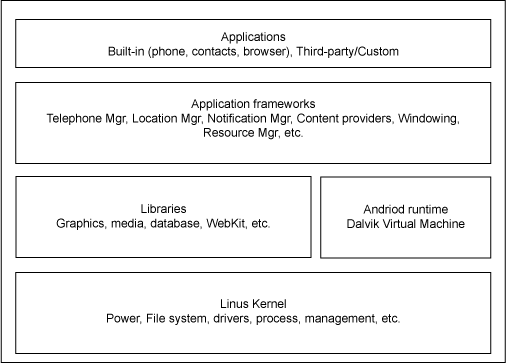
\includegraphics[width=80mm]{img/software_layers.png}}
    \caption{The structure of Android architecture.}
\end{figure}
Android applications are written in the Java programming language and run within an instance of Dalvik Virtual Machine.
\update{Proc jsme ted od vykreslovani GUI skocili zpatky k instalovani aplikace na zarizeni? Cekal bych, ze usporadani textu bude respektovat life cycle aplikace}{
%A typical application is implemented using at least one activity. 
%An activity creates a window of the application and allows the developer to render the UI.
An inseparable part of the application is AndroidManifest\@.xml file containing necessary information how to properly install it to the device 
including permissions the application needs to run.
An example of such a permission is the ability to use the phone's camera or to access the Internet.
All such requirements need to be explicitly listed in the manifest file.}
We concentrate more on activities and their development in the following sections.
\begin{figure}[h!]
    \centering{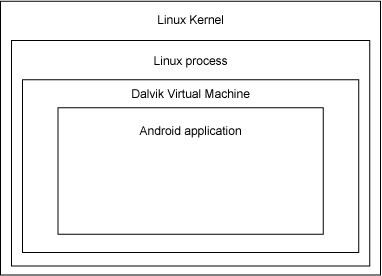
\includegraphics[width=80mm]{img/dalvik.png}}
    \caption{A typical Android application runs within an instance of Dalvik Virtual Machine on a Linux kernel.} % TODO "on a Linux kernel" se mi moc nelibi...
\end{figure}

The tools required for the development of an Android application are the Android Software Development Kit (SDK) and a Java IDE, such as Eclipse or IntelliJ IDEA. 
The Android SDK contains an Eclipse plugin supporting Android developement, documentation, sample code, and various tools, such as Android Debug Bridge used by the programmer to communicate with an application running on a device. 
% % \item The Android SDK is provided as \@.zip file including Java archive file containing all necessary classes to build an application (android\@.jar),
% the SDK documentation, a directory with sample code, Android Debug Bridge and other tools needed to build an application.

% TODO: tohle pripadne pridejme az ten text bude vyladenejsi: In the rest of this chapter we describe some of the implementing parts when developing an application.

\section{Application Components}
When an application is installed to a device, it lives in its security sandbox.
Android offers a secure environment where the applications are isolated and can safely run their code.
To each application the Linux system assign user ID number. 
Android is multi-user operating system, which means that each application is a different user with a different ID.
This number is known only to the system that sets permissions to all files so they can not be accessed by any other applications.
Each application runs unique Linux process initiated when an application or any component of it needs to be executed.
When the system needs to recover the memory or the application is not used for some time, the process shuts down.
Releasing memory works on the principe ``oldest first`` -- at first the system kills the apps that were inactive for the longest time.
Each process has its own virtual machine. This provides the security and isolation between the applications.

The security is risen by the principle of least privilege.
Due this principle an application has access only to the required components of the system. 
These requirements must be stated in the manifest file.
This protects the whole Android system and the applications from each other.

An application has several components that are used to build it.
We can divide the basic building blocks into four different groups:
\begin{itemize}
\item{Activities}
\item{Services}
\item{Content providers}
\item{Broadcast receivers}
\end{itemize}

\emph{Activity} is a screen providing the user interface.
In the activity a developer place elements such as Views, Lists, Buttons, Labels etc. 
The layout of an activity and the widgets placed in the window are described in a separate XML file (we will reveal more about user interface later).
Most of applications consist of more than one bounded activities.
Although the activities form one application, they are all independent from each other.
If another application has a permission to do so, it can start an activity of a different app.

Usually in a application there is a one main activity that shows up to the user at first after launching it.
To this one are all other activities linked.
Each Activity in android will be subclass of Activity class defined in Android SDK.

A \emph{service} is a component used to perform operations in background.
It can be invoked by an activity for example.
If the application needs to run long-term process, user can switch to another application and our process can continue to run in background.
This can be exploited to develop an application to play music or an application which needs to fetch data in the background.

A \emph{content provider} manages sharing data across the applications.
When the app is storing any data - in file system, SQLite database or any online storage, through the content provider they can be accessed or even modified from other applications.
An example when a content provider is used is an application working with the contacts database.

A \emph{broadcast receiver} is a component broadcasted by the Android system.
It usually inform applications about some basic actions such as turning the screen off, running out of battery or changes of timezone.
Applications can also initiate broadcasts to let other apps know about some action, that there some data ready to use or about completed downloading for example.
%A broadcast receiver is implemented as a subclass of an abstract class BroadcastReceiver.

From these mentioned components, activities, services and broadcasts are activated by intents.
An intent is a message to the system to invoke new activity, service or a broadcast.
It is a component activating mechanism in Android.

A very important part of an application is AndroidManifest\@.xml file, where are specified all permissions of the application.
Each Activity we create must be defined in it. Basically, every component that is used in the application must be declared in the manifest.
%code example


\section{The Activity Lifecycle}
%As we have already stated, a typical application consists of one or more activities.
Any application switches between different states of its life cycle. 
\update{jak souvisi to, ze aplikace ma aktivity s tim, ze aplikace prechazi mezi nejakymi stavy? V dalsim se pak hovori stavech aktivit a ne aplikaci}{}
Compared to desktop platforms, the programmer has only limited control over the state transitions.
\update{napsat priklad toho, co se muze stat na Androidu a nemuze se stat na desktopu}{On the desktop computer we can handle minimalizing or closing a window of an application or quite the entire app. This we can not affect on the Android device.}
The life cycle is a collection of functions operating system calls on the application while it is running.

There are five stages of the life of an application:
\begin{itemize}
\item the starting state,
\item the running state,
\item the paused state,
\item the stopped state,
\item and the destroyed state.
\end{itemize}

The starting state and the destroyed state are phases of the activity when it is not in the memory.
To launch the app, the method \emph{onCreate()} is called and eventually it is in a running state.
When the activity is in a running state it is actually on the screen seen by the user.
The activity is in foreground and handling all user interactions such as typing or touching the screen.
An activity in this state has the highest priority of getting memory in the Android Activity stack to run as quickly as possible.
It will be killed by the operating system only in extreme situations.
This transition from starting to running state is the most expensive operation in terms of battery requirements.
That is also the reason why we do not destroy every activity when it gets to the background, 
because it is probable that it is going to be called back in a while and we don't want to create all of it again.

\begin{figure}[h!]
    \centering{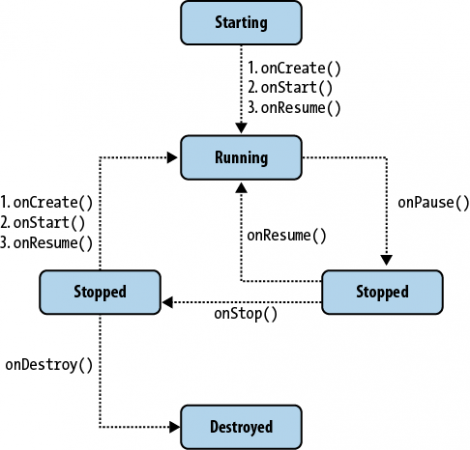
\includegraphics[width=80mm]{img/life_cycles.png}}
    \caption{Life cycles of an application.}
\end{figure}

The application is paused (in a paused state) when it is not interacting with user at the moment, but still visible on the screen.
This state does not occur that often, because most of applications cover entire screen.
But when a dialog box appears or another Activity is on the top of this one but not hiding it all, the underlying activity is partly visible and it is paused.

When the application is not visible, but still in memory, it is in a stopped state.
Then it is easy to bring it up to the front again or it can be destroyed, removed from the memory a brought to the destroyed state.

\update{Pribyly nasledujici sekce - User Interface, Sensors a Data Storage}{}

\section{User Interface}

The user interface is part and parcel of an Android application.
Basically, an application can not live without the user interface.

All elements of the user interface are built using \term{View} or \term{ViewGroup} objects.
By using them we also define the hierarchy of used components - a \term{View} can be nested within a different \term{View}.
The layout describing the visual structure of the \term{Views} of the user interface is declared in separate XML file.
Each \term{View} is represented as a XML element in it corresponding to the View class or subclass.
The user interface can be declared also right in the code of an application. 
Defining it separately make the user interface more flexible to changes without any modification of the code though.
Also, the structure of XML corresponds to the structure of UI and makes it more inspectional and easier to debug.
In the XML file declaring layout can be only one root element. 
It must be a \term{View} or \term{ViewGroup} which is \term{LinearLayout} or \term{RelativeLayout} for example.
\term{LinearLayout} is a layout that arranges the inner elements in a single row or a column depending on the set orientation, 
while in \term{RelativeLayout} are positions of its children described in relation to parent or each other.

The developer tools for Android gives us an option of creating other parts of UI beside sketching the layout such as \term{Menus}, \term{Action Bars}, \term{Dialogs} or \term{Toasts}.
There are several types of \term{Menus} such as \term{options menu} or \term{context menu}.
The \term{options menu} is an user interface component commonly used in many applications collecting menu items for an activity.
It appears when a user touches the menu button.
From the Android version 3\@.0 higher, options menu items are part of the action bar after touching the action overflow button.
The \term{context menu} is a floating menu associated with an particular element in a view that is displayed after touching the element.

\term{Action Bars} are a proper way how to navigate the user through the application.
The \term{Action Bar} is located at the top of an activity and can display the activity title, icon or other actions and items.
Some Android devices have a hardware action overflow button which opens the \term{options menu} at the bottom of an activity (as we mentioned above).
\term{Action Bars} are superiors to \term{options menus} since an \term{Action Bar} is always visible while \term{options menu} shows only on the user request.

\term{Dialog} is a small window informing the user about some action. 
Unlike the \term{Toast} it usually requires the users action before continue by confirmation or giving some additional information.
The \term{Toast} provides only feedback about some action in a small popup that disappears after a moment.


\section{Sensors}

Most Android devices have build in motion, environmental and position sensors.
Motion sensors are sensors measuring rotation along three axes and give us an opportunity to detect motion, shaking or tilt.
For measuring temperature, illumination, or humidity we use environmental sensors.
Build-in magnetometers and orientation sensors provides information about current position of a device and can be used in application for GPS navigation or map browsers.
We can access sensor events within an instance of  the \term{SensorManager} class.

\section{Data Storage}

We have several possibilities how to store our application data.
The way we choose depends on the needs and the level of privacy.
If we use private files in the application and do not want other application to access them, we prefer using the internal storage.
We read and write private data simply by using \term{FileOutputStream} and \term{FileInputStream}.

The media files such as pictures, video or audio records are usually expected to be shared and accessible from other applications.
In that case the external storage is used.
These files are readable and can be modified by user.
Methods on the \term{Environment} class provide the access to the external storage.
The function \term{getExternalStoragePublicDirectory()} depending on the argument given to it returns the path of the root directory where we can write our data, for example

\begin{itemize}
\item{../Music/}
\item{../Pictures/}
\item{../Movies/}
\item{../Download/}
\item{etc.}
\end{itemize}

As an argument we pass the type of the director we want to access, for example \term{Environment\@.DIRECTORYMUSIC}, \term{Environment. DIRECTORYPICTURES}, or \term{Environment. DIRECTORYMUSIC}. %todo: nepodarilo se mi napsat spravne typy jako"DIRECTORY_MUSIC" apod.




